\chapter{Measuring a path}
\label{ch:measuring}

A planner proposes a path; this chapter measures it. How much of the lawn
does it cut, how much twice, does the mower stay on the lawn, how long does it
take, and how far is it from the best possible? All planners of the later
chapters are judged by these measures, computed by the same function.

\section{Trajectories}

\begin{definition}{Trajectory}{trajectory}
  A \emph{trajectory} is a start pose $q_0$ and a sequence of segments
  $(\kappa_i, \ell_i, \sigma_i, m_i)$, $i = 1, \dots, k$: a constant
  curvature $\kappa_i$, a length $\ell_i \ge 0$ travelled by the middle of
  the rear axle, a direction $\sigma_i \in \{+1, -1\}$ (forward or
  reverse), and whether the blades are engaged, $m_i \in \{\text{on},
  \text{off}\}$. It is \emph{drivable} if $|\kappa_i| \le \kmax$ for all
  $i$.
\end{definition}

By Proposition~\ref{prop:arc}, the pose after each segment is known exactly,
and so is the pose at any distance along a segment. The words of
Chapter~\ref{ch:paths} are trajectories of this form, and so are straight
passes.

One simplification must be kept in mind: at the junction of two segments the
curvature jumps, which would require the steering wheel to turn
instantaneously. A real mower turns its wheels at a finite rate, so a
trajectory to be driven must later be smoothed (with clothoids, arcs whose
curvature varies linearly); this will be the subject of a later chapter.
The effect on coverage is small when the steering is fast compared with the
driving speed.

\paragraph{Blades in reverse.}
Ride-on mowers stop their blades when reversing, for safety, unless the
driver presses an override button. The flag $m_i$ models this: the code's
turns reverse with the blades off unless asked otherwise.

\section{What has been cut}

\begin{definition}{Cut area}{cut}
  The \emph{cut region} of a trajectory is the union of the blade circles
  (discs of radius $r$ around the blade centres) at all the poses where the
  blades are engaged. A point of the lawn is \emph{cut twice} if it is cut,
  then left (no blade over it), then cut again.
\end{definition}

The simulator computes the cut region on the raster of
Section~\ref{sec:raster}: it samples the trajectory finely, and at each
sample marks every cell whose centre lies inside a blade circle.

\begin{proposition}{Sampling step}{step}
  Let $\rho_{\max}$ be the largest distance from $P$ to a point of the blade
  circles. If the middle of the rear axle advances by at most
  \[
    \Delta s = \frac h2 \,\frac{\Rmin}{\Rmin + \rho_{\max}}
  \]
  between two samples, no point of a blade circle moves more than $h/2$
  between them, so no cell crossed by a blade can be missed.
\end{proposition}

\begin{proof}
  On an arc of radius $R \ge \Rmin$, a point $Q$ of the mower moves at
  $|Q - C| / R$ times the speed of $P$ (Proposition~\ref{prop:icr}), and by
  the triangle inequality $|Q - C| \le |C - P| + |P - Q| \le R +
  \rho_{\max}$. Its speed ratio is therefore at most $(R + \rho_{\max})/R
  \le (\Rmin + \rho_{\max})/\Rmin$, since this decreases with $R$. Straight
  ahead the ratio is 1. While $P$ advances by $\Delta s$, $Q$ moves by at
  most $\Delta s\,(\Rmin + \rho_{\max})/\Rmin = h/2$.
\end{proof}

\begin{example}{The default sampling step}{stepnum}
  The farthest blade point is the tip of a blade, at
  $\rho_{\max} = \sqrt{d^2 + y_1^2} + r = \sqrt{0.55^2 + 0.235^2} + 0.25 =
  0.598 + 0.25 = \SI{0.848}{\metre}$ from $P$. With $h = \SI{0.05}{\metre}$
  and $\Rmin = \SI{1.430}{\metre}$:
  \[
    \Delta s = \frac{0.05}{2} \times \frac{1.430}{1.430 + 0.848}
    = 0.025 \times 0.628 = \SI{0.0157}{\metre},
  \]
  about 64 samples per metre.
\end{example}

\paragraph{Counting passes.}
For each cell, the simulator lists the distances along the trajectory at
which it was cut. A pass of the deck over a cell gives a run of close
distances; a new pass starts when two successive cuts are separated by more
than the length of the deck plus a margin (\SI{0.66}{\metre} by default).
The \emph{area cut twice} is the area of the cells cut in two passes or more.
Reversing straight back over a strip just cut counts as a second pass, as it
should, as soon as the deck has left the cell in between.

\paragraph{Accuracy.}
Two errors remain: the raster (Theorem~\ref{thm:rastererror}), and the
decision ``centre inside a blade circle'' for the cells on the edge of the
cut band. Both are of the order of $h$ times the length of the edges, and
mostly cancel when the edges cross the grid at an angle
(Figure~\ref{fig:raster}). The tests of the code check the simulator against
exact areas: a full circle at full lock (an annulus,
Example~\ref{ex:uncut}) within 1\%, and a straight pass at 17° within 0.5\%.

\section{Staying on the lawn}

\begin{definition}{Collision}{collision}
  The mower's \emph{footprint} is the union of its body and its deck housing
  (Figure~\ref{fig:mower}). A sample of a trajectory is a \emph{collision}
  if part of the footprint is off the lawn: outside the border or over a
  hole. A trajectory is \emph{feasible} if it is drivable and has no
  collision.
\end{definition}

The simulator places points every $h$ along the outlines of the body and of
the deck housing, moves them to each sample pose (Definition~\ref{def:pose}),
and checks that they all fall on lawn cells. An obstacle smaller than $h$
could slip between two points; for lawns this is not a limitation, since a
tree trunk or a post is much larger than \SI{5}{\centi\metre}. A real robot
also needs a safety margin for its localisation error; a later chapter will
add it.

\section{How short can a complete path be?}

On the grid, a path that visits $N$ cells needs at least $N - 1$ moves. The
continuous analogue bounds the length of any path that cuts the whole lawn.

\begin{theorem}{Lower bound on the mowing length}{lowerbound}
  Let $a_0$ be the area under the blades at standstill, and
  \[
    w_{\max} = \max_{|\kappa| \le \kmax} \weff(\kappa)
  \]
  the largest area swept per metre (Proposition~\ref{prop:weff}). A
  drivable trajectory whose blades are engaged $n$ times and travel a
  distance $\ell_{\mathrm{mow}}$ while engaged cuts an area of at most
  \[
    n\,a_0 + w_{\max}\,\ell_{\mathrm{mow}} .
  \]
  Consequently, a trajectory that cuts the whole lawn, of area $A$, satisfies
  \[
    \ell_{\mathrm{mow}} \;\ge\; \frac{A - n\,a_0}{w_{\max}} .
  \]
\end{theorem}

\begin{proof}
  When the blades are engaged, they cut at once the discs under them, an
  area at most $a_0$. While they stay engaged and $P$ advances by $ds$ on a
  segment of curvature $\kappa$, the area cut grows by at most
  $\weff(\kappa)\,ds \le w_{\max}\,ds$ (Proposition~\ref{prop:weff}, whose
  proof holds forward and in reverse, since the swept sector is the same).
  At a cusp the mower stops and cuts nothing new. Adding over the $n$
  engagements and over the segments gives the first inequality. If the whole
  lawn is cut, $A \le n\,a_0 + w_{\max}\,\ell_{\mathrm{mow}}$, which is the
  second.
\end{proof}

\begin{example}{The rectangle}{boundrect}
  For the \SI{20}{\metre} $\times$ \SI{12}{\metre} lawn ($A =
  \SI{240}{\metre\squared}$), with two blade discs of radius
  \SI{0.25}{\metre} ($a_0 \le 2\pi \times 0.25^2 = \SI{0.393}{\metre
  \squared}$), $w_{\max} = \weff(\kmax) = \SI{1.0065}{\metre}$
  (Example~\ref{ex:weffnum}) and the blades engaged once:
  \[
    \ell_{\mathrm{mow}} \ge \frac{240 - 0.393}{1.0065}
    = \SI{238.1}{\metre}.
  \]
  If the mower only drove straight, $w_{\max}$ would be $w$ and the bound
  $240/0.97 = \SI{247.4}{\metre}$: the turns, which sweep a little faster,
  lower the guaranteed minimum.
\end{example}

\begin{definition}{Efficiency}{efficiency}
  The \emph{efficiency} of a trajectory is
  \[
    \eta = \frac{(A_{\mathrm{cut}} - n\,a_0)/w_{\max}}{\ell_{\mathrm{mow}}},
  \]
  the lower bound for the area it actually cut, with its $n$ engagements,
  divided by the distance it mowed. By Theorem~\ref{thm:lowerbound},
  $\eta \le 1$.
\end{definition}

\begin{inwords}
  The bound says: the blades cannot cut more than about one metre of width
  per metre driven, so a lawn of \SI{240}{\metre\squared} needs at least
  \SI{238}{\metre} of mowing. It is a guaranteed minimum, not a target: no
  real path reaches it, because the turns at the ends of the passes overlap
  and the border needs extra care. The efficiency says how much of the
  mowing distance did useful work.
\end{inwords}

\section{Time}

The time of a trajectory is that of Definition~\ref{def:time}: each segment
at the speed for its kind (straight forward, arc forward, reverse), plus a
fixed time at each change of direction. Time is the measure that matters to
the owner of the lawn; the area cut twice and the length are its main
causes.

\section{A first experiment: back and forth on a rectangle}

To exercise the simulator, the code has a deliberately naive trajectory
(\code{mowersim/demo.py}, not a planner): parallel passes along the length of
the lawn, \SI{0.92}{\metre} apart (the cutting width minus \SI{5}{\centi
\metre} of overlap), joined by the fastest Reeds--Shepp turn of
Section~\ref{sec:nextpass}, blades off in reverse. It comes in two
versions:

\begin{description}
  \item[Passes to the edge.]
    \leavevmode\\
    The passes run until the front of the mower reaches the border.
  \item[Room for the turns.]
    \leavevmode\\
    The passes stop early enough for the whole turn, mower included, to stay
    on the lawn. The code computes this room by driving the turn and
    measuring how far the footprint goes beyond the end of the pass
    (\SI{2.46}{\metre} ahead of the rear axle, against \SI{1.55}{\metre} for
    the mower standing still), and how far it bulges sideways beyond the next
    pass (\SI{1.64}{\metre}).
\end{description}

\begin{figure}[ht]
  \centering
  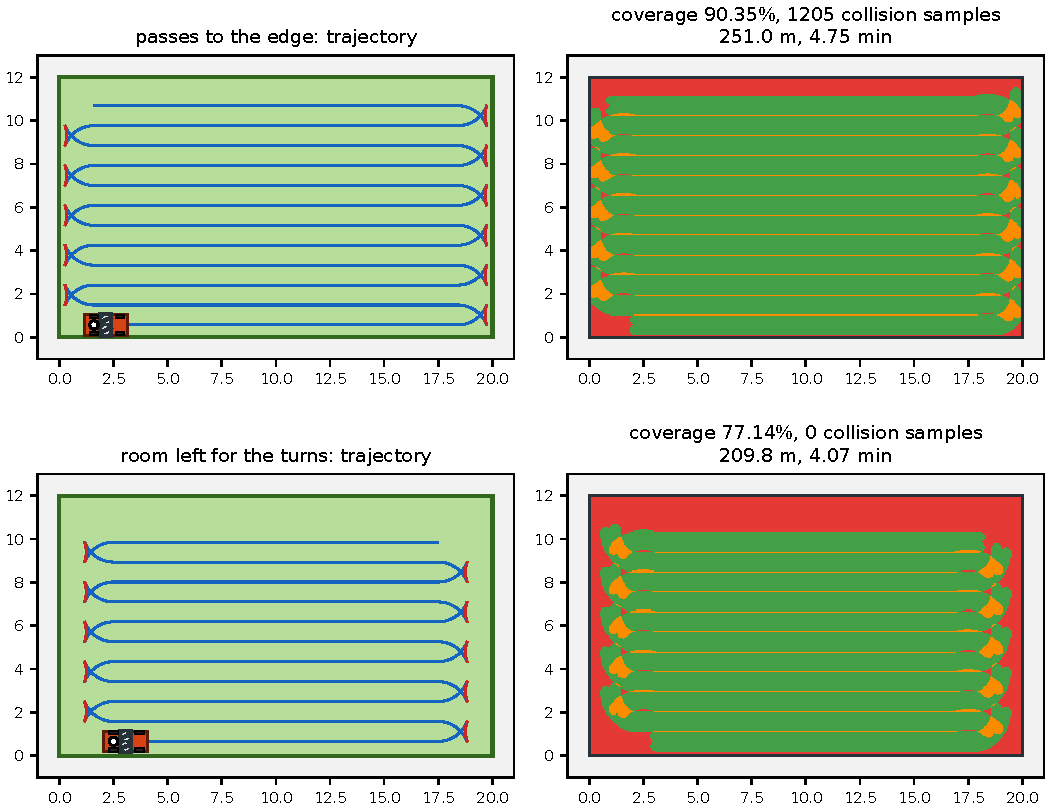
\includegraphics[width=\textwidth]{figures/demo}
  \caption{Back and forth on the \SI{20}{\metre} $\times$ \SI{12}{\metre}
    lawn, with the default mower. Left: the path of the middle of the rear
    axle (blue forward, red reverse) and the mower at its start. Right: the
    cut grass (green: once, orange: twice or more, red: missed). Top: the
    passes run to the edge, and the turns drive the mower off the lawn.
    Bottom: the passes leave room for the turns; the mower stays on the lawn,
    but strips at both ends and along the top are not cut.}
  \label{fig:demo}
\end{figure}

\begin{center}
\begin{tabular}{@{}lrr@{}}
  \toprule
  & passes to the edge & room for the turns \\
  \midrule
  coverage & 90.4\% & 77.1\% \\
  missed area & \SI{23.2}{\metre\squared} & \SI{54.9}{\metre\squared} \\
  area cut twice & \SI{17.0}{\metre\squared} & \SI{14.6}{\metre\squared} \\
  collision samples & 1205 & 0 \\
  length (of which reverse) & \SI{251.0}{\metre} (\SI{10.9}{\metre}) &
    \SI{209.8}{\metre} (\SI{9.9}{\metre}) \\
  time & \SI{4.75}{\minute} & \SI{4.07}{\minute} \\
  efficiency $\eta$ & 0.878 & 0.899 \\
  \bottomrule
\end{tabular}
\end{center}

Neither version is acceptable. Running the passes to the edge cuts most of
the lawn but drives off it at every turn: on a real lawn, into the flower bed
or the fence. Leaving room for the turns keeps the mower on the lawn but
leaves almost a quarter of it uncut, in the strips where it turns. The area
cut twice is where consecutive turns overlap.

This is the problem every real mowing pattern solves first: the mower needs a
\emph{headland}, a band along the border where it can turn, and the headland
itself must be mowed, by passes that follow the border. Designing the
headland passes, choosing the direction of the main passes and joining
everything with feasible turns is the subject of the next chapter.

\begin{incode}
  \code{mowersim/kinematics.py}: \code{Trajectory}, \code{Segment},
  \code{Trajectory.sample}. \code{mowersim/coverage.py}: \code{evaluate}
  returns a \code{Result} with every measure of this chapter;
  \code{sample\_step} is Proposition~\ref{prop:step}, \code{cut\_cells} counts
  the passes, \code{collisions} checks the footprint,
  \code{length\_lower\_bound} is Theorem~\ref{thm:lowerbound}.
  \code{python -m mowersim demo lawns/rectangle.json -{}-png demo.png} runs the
  experiment (\code{-{}-no-room} for the passes to the edge, \code{-{}-gif} for an
  animation).
\end{incode}
